\documentclass[12pt]{article}
\usepackage[left=1cm, right=1cm, top=2cm,bottom=1.5cm]{geometry} 

\usepackage[parfill]{parskip}
\usepackage[utf8]{inputenc}
\usepackage[T2A]{fontenc}
\usepackage[russian]{babel}
\usepackage{enumitem}
\usepackage[normalem]{ulem}
\usepackage{amsfonts, amsmath, amsthm, amssymb, mathtools}

\usepackage{fancyhdr}
\pagestyle{fancy}
\renewcommand{\headrulewidth}{1.5pt}
\renewcommand{\footrulewidth}{1pt}

\usepackage{graphicx}
\usepackage[figurename=Рис.]{caption}
\usepackage{subcaption}
\usepackage{float}

%%Наименование папки откуда забирать изображения
\graphicspath{ {./images/} }

%%Изменение формата для ввода доказательства
\renewcommand{\proofname}{$\square$  \nopunct}
\renewcommand\qedsymbol{$\blacksquare$}

\addto\captionsrussian{%
	\renewcommand{\proofname}{$\square$ \nopunct}%
}
%% Римские цифры
\newcommand{\RN}[1]{%
	\textup{\uppercase\expandafter{\romannumeral#1}}%
}


\theoremstyle{definition}
\newtheorem{defn}{Опр:}
\newtheorem{rem}{Rm:}
\newtheorem{prop}{Утв.}
\newtheorem{exrc}{Упр.}
\newtheorem{lemma}{Лемма}
\newtheorem{theorem}{Теорема}
\newtheorem{corollary}{Следствие}

\newenvironment{cusdefn}[1]
{\renewcommand\thedefn{#1}\defn}
{\enddefn}



\DeclareRobustCommand{\divby}{%
	\mathrel{\text{\vbox{\baselineskip.65ex\lineskiplimit0pt\hbox{.}\hbox{.}\hbox{.}}}}%
}


\newcommand{\smallerrel}[1]{\mathrel{\mathpalette\smallerrelaux{#1}}}
\newcommand{\smallerrelaux}[2]{\raisebox{.1ex}{\scalebox{.75}{$#1#2$}}}

\newcommand{\smallin}{\smallerrel{\in}}
\newcommand{\smallnotin}{\smallerrel{\notin}}

\newcommand*{\medcap}{\mathbin{\scalebox{1.25}{\ensuremath{\cap}}}}%
\newcommand*{\medcup}{\mathbin{\scalebox{1.25}{\ensuremath{\cup}}}}%

\begin{document}
	\lhead{Математический анализ - I}
	\chead{Шапошников С.В.}
	\rhead{Лекция - 14}
	
\begin{defn}
	 $K \subset \mathbb{R}$ называется \uwave{компактом}, если $\forall \! \underset{\text{откр. мн-ва}}{\{\mathcal{U}_\alpha\}} \colon \bigcup\limits_\alpha \mathcal{U}_{\alpha} \supset K, \, \exists \, \mathcal{U}_{\alpha_1}, \dotsc, \mathcal{U}_{\alpha_N} \colon K \subset \bigcup\limits_{n = 1}^{N} \mathcal{U}_{\alpha_n}$.
\end{defn}
	
\begin{prop}
	$K$ - компакт $\Leftrightarrow K$ - ограничено и замкнуто. 
\end{prop}
	
\begin{theorem}
	$K$ - компакт $\Leftrightarrow \forall \{x_n\}_{n=1}^{\infty} \in K, \,\exists$ подпоследовательность $\{x_{n_k}\} \colon x_{n_k} \to x \in K$.
\end{theorem}
	
\begin{proof}\hfill\\
	$(\Rightarrow)$ Пусть $K$ - компакт. Так как $K$ - ограничено, то $\exists \, [a,b] \supset K$. Пусть $\{x_n\} \in K$, тогда $x_n \in [a,b]$. По теореме Больцано $\exists \, x_{n_k} \to x$. Так как $K$ - замкнутое множество, то $x \in K$.
	
	$(\Leftarrow)$ Пусть $\forall \{x_n\}\in K, \,\exists \, x_{n_k} \to x \in K$. Докажем, что $K$ - компакт. 
	
	Если $K$ не ограниченно сверху, то $\exists \, x_n \in K \colon x_n \to +\infty$. Из этой последовательности нельзя выбрать сходящуюся подпоследовательность (так как все ее подпоследовательности будут уходить в $+\infty$).
	
	Если $K$ не ограниченно снизу, то $\exists \, x_n \in K \colon x_n \to -\infty$. Из этой последовательности нельзя выбрать сходящуюся подпоследовательность (так как все ее подпоследовательности будут уходить в $-\infty$).
	
	Следовательно $K$ - ограниченно. Проверим, что $K$ - замкнуто.
	
	Пусть $x_n \in K$ и $x_n \to x$, покажем, что $x \in K$. По условию $\exists \, x_{n_k} \to x_0 \in K$, но $x_0 = x$, так как предел подпоследовательности обязательно совпадает с пределом сходящейся последовательности.
\end{proof}

\subsection*{Множество Кантора}

\uline{Построение Множества Кантора}:

$F_1$: Отрезок $[0,1]$, делится на три равные части и выбрасывается середина $\Rightarrow$  $F_1 = [0,\tfrac{1}{3}] \cup [\tfrac{2}{3}, 1]$.

\begin{figure}[H]
	\centering
	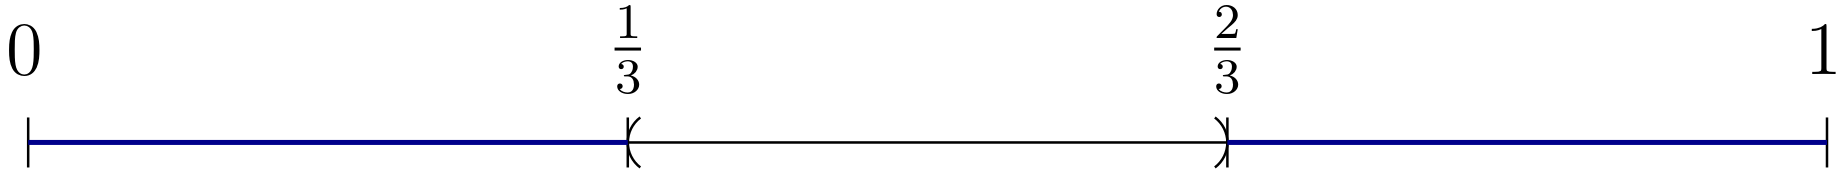
\includegraphics[width=0.65\textwidth]{14_1.png}
	\caption{Множество $F_1 = [0,\tfrac{1}{3}] \cup [\tfrac{2}{3}, 1]$.}
	\label{14_1}
\end{figure}

$F_2$: Каждый из отрезков $F_1$ делится также на три части и в каждом из них выбрасывается середина.

\begin{figure}[H]
	\centering
	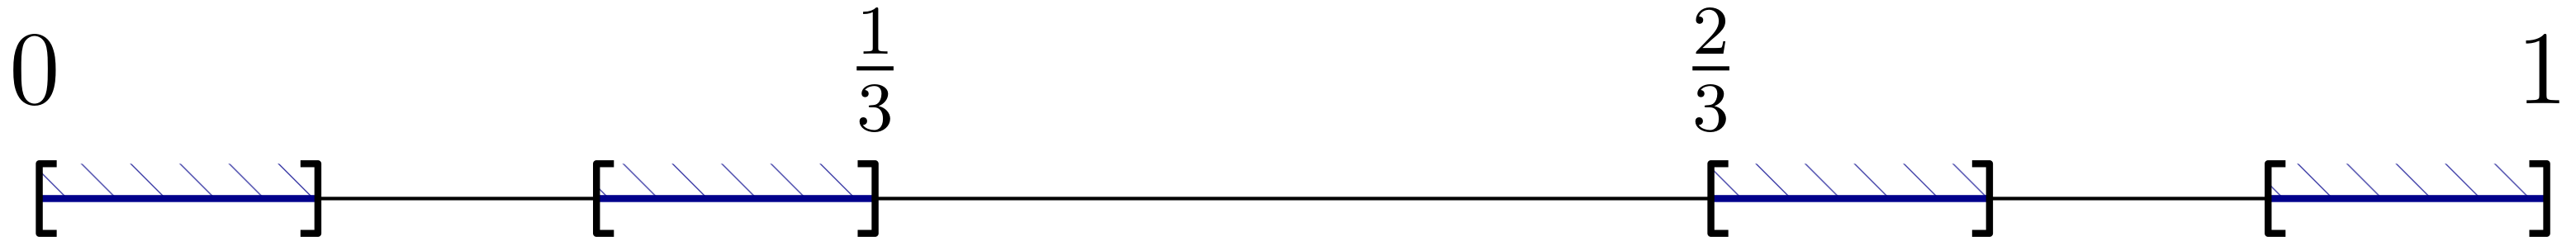
\includegraphics[width=0.65\textwidth]{14_2.png}
	\caption{Множество $F_2$.}
	\label{14_2}
\end{figure}

Далее по аналогии. Таким образом, любое $F_n$ - конечное объединение отрезков $\Rightarrow F_n$ - замкнутые. Также важно отметить, что: $F_1 \supset F_2 \supset F_3 \supset \dotsc \supset F_n \supset \dotsc$ - множества вложенные.

Рассмотрим длины отрезков: $|F_1| = \frac{2}{3}$, $|F_2| = \frac{4}{9}$,  $|F_n| = \big(\frac{2}{3}\big)^n = $ сумма длин, составляющих их отрезков. Видно, что $$|F_n| = \bigg(\frac{2}{3}\bigg)^n \xrightarrow[n \to \infty]{} 0$$ Тогда сумма длин выбрасываемых интервалов стремится к $1$. Но это не весь интервал.

\begin{defn}
	\uwave{Множество Кантора} $C = \bigcap\limits_{n=1}^{\infty}F_n$.
\end{defn}

В множестве Кантора точно будут концы выбрасываемых интервалов, так как дополнение к этому множеству это набор интервалов, куда эти концы никогда не входят.
\begin{figure}[H]
	\centering
	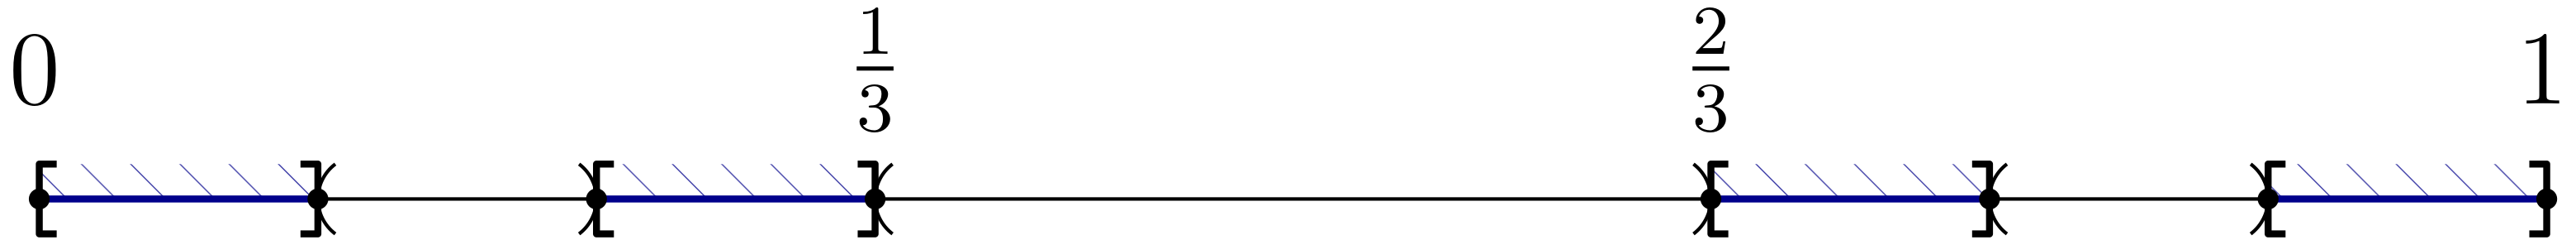
\includegraphics[width=0.65\textwidth]{14_3.png}
	\caption{Множество Кантора.}
	\label{14_3}
\end{figure}

На самом деле, там останется континуум точек.

\begin{prop}Справедливы следующие утверждения, относительно множества Кантора:
	\begin{enumerate}[label={(\arabic*)}]
		\item $C$ - замкнуто и ограниченно (компакт);
		\item $C$ - континуально;
		\item ``По длине'' (при $n \to \infty$) остался 0;
	\end{enumerate}
\end{prop}

\begin{proof}\hfill
	\begin{enumerate}[label={(\arabic*)}]
		\item Ограниченно - по условию, поскольку все производилось внутри отрезка $[0,1]$. Множество ограниченно, поскольку любое пересечение замкнутых множеств - замкнуто $\Rightarrow$ получим компакт. 
		\item Будем кодировать точки, которые останутся в Канторовском множестве. Взяли отрезок, выбросили середину. Левой части сопоставили $0$, правой части - $2$.
		
		\begin{figure}[H]
			\centering
			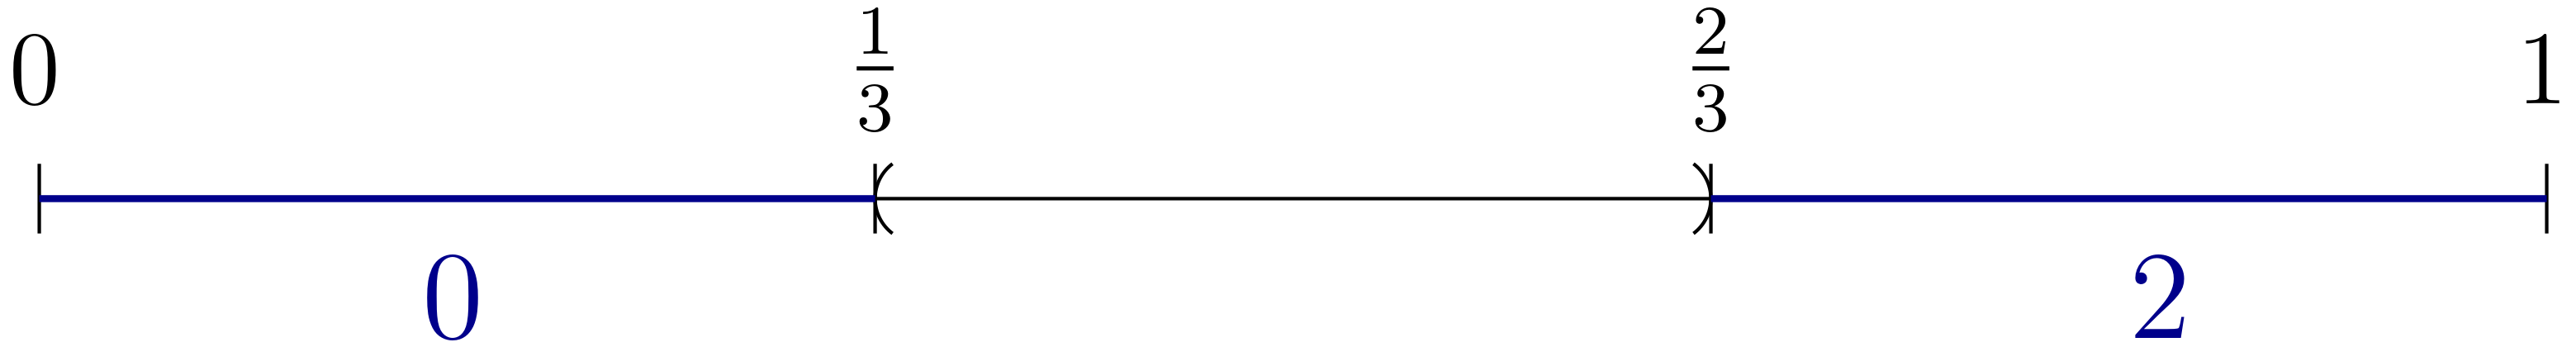
\includegraphics[width=0.65\textwidth]{14_4.png}
			\caption{Кодирование множества Кантора.}
			\label{14_4}
		\end{figure}
		
		Продолжаем нумеровать интервалы. Получится, что всякая точка $x \in C$ Канторовского множества записалась в виде последовательности $0$ и $2$: $0222\dotsc\;$. 
		
		\begin{figure}[H]
			\centering
			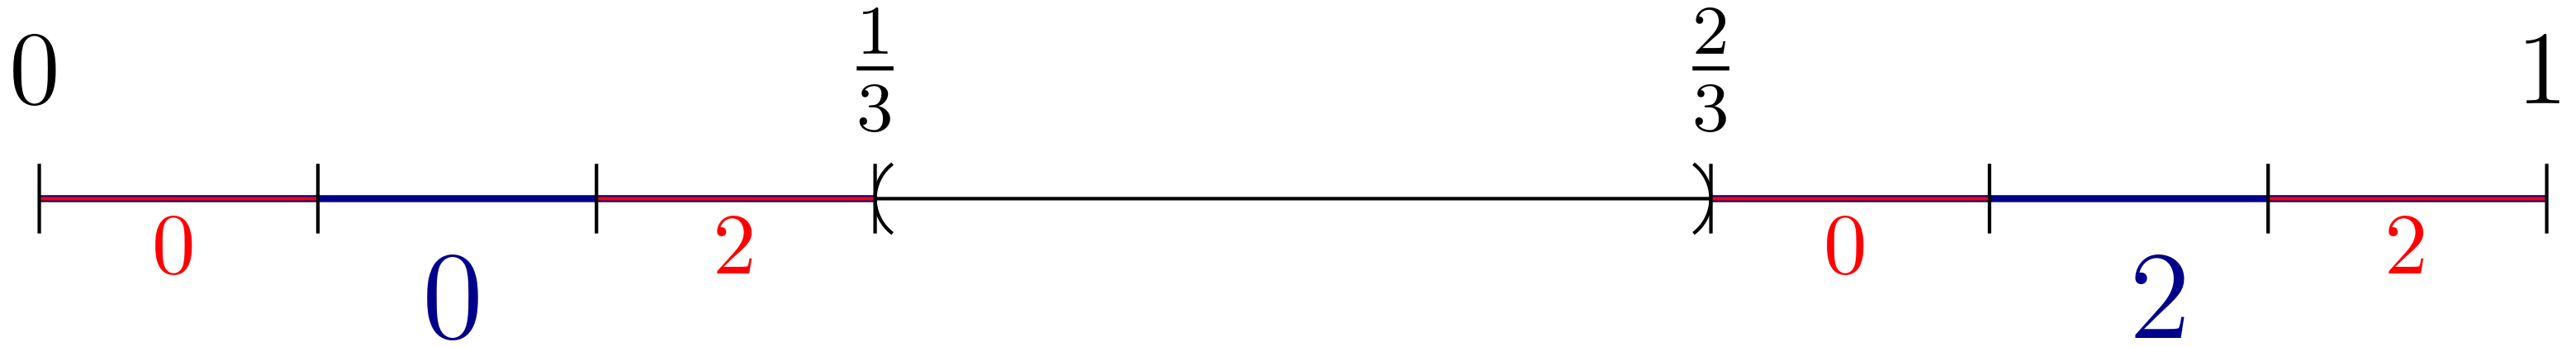
\includegraphics[width=0.65\textwidth]{14_5.png}
			\caption{Кодирование множества Кантора.}
			\label{14_5}
		\end{figure}
		
		Такая запись однозначна, так как если две точки отличаются, то поскольку длины отрезков стремятся к $0$, то рано или поздно одна точка окажется в одной трети, другая - в другой. 
		
		Для каждой такой записи существует точка Канторовского множества по теореме о вложенных отрезках.
		
		Таким образом, точки $C$ взаимно однозначно соответствуют последовательностям $0$ и $2$. Значит этих точек столько же, сколько последовательностей $0$ и $2$, а их столько же, сколько последовательностей $0$ и $1$, а значит их континуум.
		
		\item Длина интервалов множества Кантора: $|F_n| = \big(\frac{2}{3}\big)^n \xrightarrow[n \to \infty]{} 0$.
	\end{enumerate}
\end{proof}

\begin{exrc}\hfill
	\begin{enumerate}[label={\arabic*)}]
		\item Показать $\frac{1}{4} \in C$ (разложить в троичной системе);
		\item Множество предельных точек $C = С$ (это совершенные множества - привести примеры);
		\item Доказать $C + C = [0,2]$
	\end{enumerate}
\end{exrc}
\newpage

\section*{Предел функции и его свойства}

Пусть $D \subset \mathbb{R}, \, f \colon D \to \mathbb{R}$ - функция. Предположим, что $a$ - предельная точка $D$ ($a\notin D$ или $a \in D$).

\begin{defn}\textbf{(Гейне)}:
	Число $b$ называется \uwave{пределом функции} $f$ при $x \to a$ (по множеству $D$), если\\ 
	$\forall \{x_n\} \in D, \, x_n \to a \wedge x_n \neq a$ верно, что $f(x_n) \to b$.
\end{defn}

\begin{figure}[H]
	\centering
	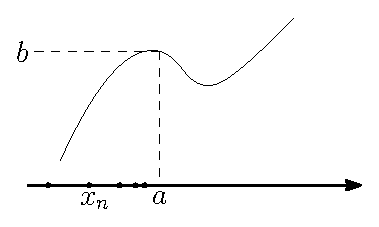
\includegraphics[width=0.35\textwidth]{14_6.eps}
	\caption{Предел функции при $x \to a$.}
	\label{14_6}
\end{figure}


Зачем есть требование $x_n \neq a$? Рассмотрим следующий пример.

\textbf{Пример}: 

\begin{figure}[H]
	\centering
	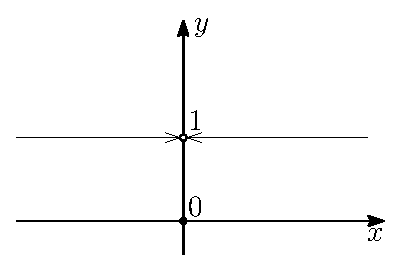
\includegraphics[width=0.35\textwidth]{14_7.eps}
	\caption{Предел функции при $x \to 0$.}
	\label{14_7}
\end{figure}

При $x \to 0$, функция стремится к $1$. Но если не поставить $x\neq a$, то у такой функции вообще может не быть предела. Взяв, к примеру, последовательность $x_n \colon 1,\,0,\,\frac{1}{2},\, 0, \dotsc\;$.

Требуем, чтобы $a$ была предельной точкой, так как иначе таких последовательностей может вообще не оказаться. Если $a$ - не предельная точка, то у неё есть окрестность в которой отличной от неё точек лишь конечный набор.

\begin{rem}
	Как установить расходящуюся последовательность? Можно либо взять последовательность при которой $x_n \to a$, но $f(x_n) \not\to b$, либо предъявить несколько последовательностей $x_n \to a$, $y_n \to a$ и \\
	$f(x_n) \to b \wedge f(y_n) \to c$, где $b \neq c$.
\end{rem}

\uline{Обозначение}: Пишут 
$$b = \lim\limits_{D \ni x\to a}f(x) = \lim\limits_{ x\to a}f(x)$$

\begin{rem}	Ничего не поменяется в определении предела функции, если в качестве $a$ взять $\pm\infty$. Только необходимо, чтобы они оказались предельными точками.
	\begin{enumerate}[label={(\arabic*)}]
		\item Если $D$ не ограниченно сверху, то в качестве $a$ можно взять $+\infty$.
		\item Если $D$ не ограниченно снизу, то в качестве $a$ можно взять $-\infty$.
	\end{enumerate}
\end{rem}

Все свелось к последовательностям. Поэтому будем переносить свойства с пределов последовательностей на пределы функций.

\begin{theorem}
	Количество пределов функции при $x \to a$ $\leq 1$.
\end{theorem}

\begin{proof}
	Предположим, что $\lim\limits_{x \to a} f(x) = b$ и  $\lim\limits_{x \to a} f(x) = c$. По определению для всякой последовательности $x_n \colon x_n \to a \wedge x_n \neq a$ верно $f(x_n) \to b \wedge f(x_n) \to c$. Пределов последовательности $\leq 1 \Rightarrow b = c$. 
\end{proof}

\begin{rem}
	В доказательстве данной теоремы важно, что такая последовательность $x_n$ вообще есть. Но это условие выполнено, так как $a$ - предельная точка $D$, то есть всегда можно выбрать последовательность, которая к ней сходится.
\end{rem}

\textbf{Пример}: У данной функции:
\begin{figure}[H]
	\centering
	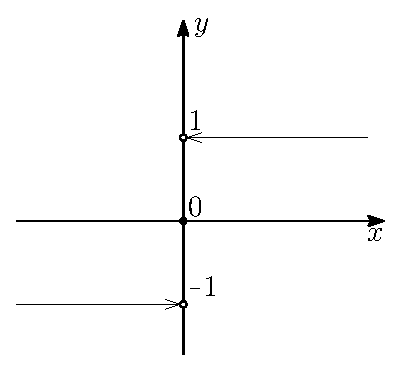
\includegraphics[width=0.25\textwidth]{14_8.eps}
	\caption{Не существование предела функции $f(x)$ при $x \to 0$.}
	\label{14_8}
\end{figure}
предела $ \lim\limits_{x \to 0} f(x)$не существует. Возьмем $x_n = \frac{1}{n}, \, f(x_n) \to 1$, а потом возьмем $x_n = -\frac{1}{n}, \, f(x_n) \to -1$. Если бы предел был, то он бы совпадал.

\begin{theorem}\textbf{(Переход к пределу в неравенствах)}:
	Пусть $f\colon D \to \mathbb{R}, \, g\colon D \to \mathbb{R}$ и $a$ - предельная точка $D$.  Предположим, что $\lim\limits_{x \to a}f(x) = b$, $\lim\limits_{x\to a}g(x) = c$ и $\exists \, \mathcal{U}^\prime(a) \colon f(x) \leq g(x), \, \forall x \in \mathcal{U}^\prime(a) \cap D$ (пересечение не пусто, так как $a$ - предельная точка $D$), тогда $b \leq c$.
\end{theorem}

\begin{proof}
	Пусть $x_n \to a \wedge x_n \neq a, \, x_n \in D$. По определению предела функции: $f(x_n) \to b$, $g(x_n) \to c$. По определению предела последовательности $\exists \, N \colon \forall n > N, \, x_n \in \mathcal{U}^\prime(a)$ и так как $x_n \in D \Rightarrow x_n \in \mathcal{U}^\prime(a) \cap D \Rightarrow$\\
	$\Rightarrow f(x_n) \leq g(x_n), \, \forall n>N$. По свойству предела последовательности $b \leq c$.
\end{proof}

Точно также, как и для последовательностей пределы всегда переводят неравенства в нестрогие. 

\begin{theorem}\textbf{(О двух полицейских)}:
	Пусть $f\colon D \to \mathbb{R}, \, g\colon D \to \mathbb{R}, \, h\colon D \to \mathbb{R}$ и $a$ - предельная точка $D$. Предположим, что $\lim\limits_{x \to a}f(x) = \lim\limits_{x\to a}g(x) = b$ и $\exists \, \mathcal{U}^\prime(a) \colon f(x) \leq h(x) \leq g(x), \, \forall x \in \mathcal{U}^\prime(a) \cap D$, тогда $\exists \, \lim\limits_{x \to a} h(x) = b$.
\end{theorem}

\begin{proof}
	Для всякой последовательности $x_n \in D \colon x_n \to a \wedge x_n \neq a$ верно, что $f(x_n) \to b$, $g(x_n) \to b$ и $\exists \, N \colon \forall n >N, \, x_n \in \mathcal{U}^\prime(a) \cap D$ и значит $f(x_n) \leq h(x_n) \leq g(x_n)$. По теореме о двух полицейских для последовательностей $h(x_n) \to b$.
\end{proof}

\begin{theorem}\textbf{(Арифметика пределов)}:
	Пусть $f\colon D \to \mathbb{R}, \, g\colon D \to \mathbb{R}$ и $a$ - предельная точка $D$. Предположим, что $\lim\limits_{x \to a}f(x) = b$, $\lim\limits_{x\to a}g(x) = c$, тогда:
	\begin{enumerate}[label={(\arabic*)}]
		\item $\lim\limits_{x \to a} \big(f(x) + g(x)\big) = b + c$;
		\item $\lim\limits_{x \to a} \big(f(x) \cdot g(x)\big) = b \cdot c$;
		\item Если $g \neq 0$ на множестве $D$ и $c \neq 0$, то $\lim\limits_{x \to a} \dfrac{f(x)}{g(x)} = \dfrac{b}{c}$;
	\end{enumerate}
\end{theorem}

\begin{proof}\hfill
	\begin{enumerate}[label={(\arabic*)}]
		\item Для всякой последовательности $x_n \in D \colon x_n \to a \wedge x_n \neq a$ верно, что $f(x_n) \to b$, $g(x_n) \to c$. По арифметике пределов последовательности $f(x_n) + g(x_n) \to b + c$.
		\item Для всякой последовательности $x_n \in D \colon x_n \to a \wedge x_n \neq a$ верно, что $f(x_n) \to b$, $g(x_n) \to c$. По арифметике пределов последовательности $f(x_n) \cdot g(x_n) \to b \cdot c$.
		\item Для всякой последовательности $x_n \in D \colon x_n \to a \wedge x_n \neq a$ верно, что $f(x_n) \to b$, $g(x_n) \to c$ и $g(x_n) \neq 0, \, c \neq 0$. По арифметике пределов последовательности $\dfrac{f(x_n)}{g(x_n)} \to \dfrac{b}{c}$.
	\end{enumerate}
\end{proof}

\begin{theorem} \textbf{(Предел сложной функции)}:
	 Пусть $D \subset \mathbb{R}$ и $E \subset \mathbb{R}$, $f\colon D \to E, \, g\colon E \to \mathbb{R}$. Пусть $a$ - предельная точка $D$ и $b$ - предельная точка $E$ и $\exists \, \mathcal{U}^\prime(a) \colon \forall x \in \mathcal{U}^\prime(a) \cap D, \, f(x) \neq b$. Предположим, что $\lim\limits_{x \to a} f(x) = b$ и $\lim\limits_{y \to b} g(y) = c$, тогда $\lim\limits_{x \to a} g\big(f(x) \big) = c$.
\end{theorem}

\begin{proof}
	$\forall x_n \to a \wedge x_n \neq a, \, f(x_n) \to b$, кроме того $\exists \, N \colon \forall n > N, \, f(x_n) \neq b$. Таким образом последовательность $f(x_{N+1}), \dotsc, \, f(x_n), \dotsc$ - сходится к $b$ и никакой из её элементов $\neq b \Rightarrow$\\
	последовательность $\Rightarrow g\big(f(x_{N+1})\big), \dotsc, \, g\big(f(x_n)\big), \dotsc \to c \Rightarrow g\big(f(x_n) \big) \to c$.
\end{proof}

\begin{rem}
	\uline{Важно}, что есть условие $\exists \, \mathcal{U}^\prime(a) \colon \forall x \in \mathcal{U}^\prime(a) \cap D, \, f(x) \neq b$. Рассмотрим к примеру функцию $f(x) = x \sin{\frac{1}{x}}, \, f(0) = 0$. $\lim\limits_{x \to 0}f(x_n) = 0$, так как $|f(x)| \leq |x|, \, x_n \to 0 \Rightarrow |x_n| \to 0 \Rightarrow f(x_n) \to 0$ и $\lim\limits_{y\to 0}g(y) = 1$, но у композиции предела нет: $\nexists \, \lim\limits_{x \to 0} g\big( f(x)\big)$.
	\begin{figure}[H]
		\begin{subfigure}[b]{0.5\textwidth}
			\centering
			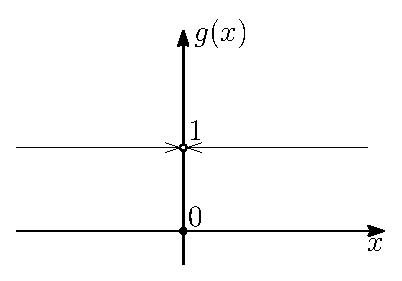
\includegraphics[width=0.5\textwidth]{14_9.eps}
			\caption{Функция $g(x)$.}
			\label{14_9}
		\end{subfigure}%
		\begin{subfigure}[b]{0.5\textwidth}
			\centering
			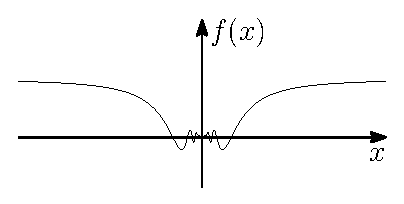
\includegraphics[width=0.5\textwidth]{14_10.eps}
			\caption{Функция $f(x)$.}
			\label{14_10}
		\end{subfigure}
	\end{figure}
	Возьмем последовательность нулей функции $f(x)$: $x_n = \frac{1}{\pi n}, \, f(x_n) = 0, \, g\big( f(x_n)\big) = 0$.\\
	Возьмем последовательность положительных значенией $f(x)$:  $x_n =\dfrac{1}{\frac{\pi}{2} + 2\pi n}, \, f(x_n) = 0, \, g\big( f(x_n)\big) = 1 \Rightarrow$ нет предела. Так получилось, поскольку $f(x)$ принимала предельные значения $b$.
\end{rem}

\end{document}